\section{Introduction}
There is a \textbf{theory} which states that \textit{if ever anyone discovers exactly what the Universe is for and why it is here, it will instantly disappear and be replaced by something even more bizarre and inexplicable} \cite{miller90introduction}. For more details look at the Figure \ref{fig:universe}.

There is another \textbf{theory} which states that \textit{this has already happened} \cite{aberer03chatty}. The authors present the stars, show a nice picture of the moon, and laugh out loud because they drink a lot of alcohol.


\begin{figure}[h!]
\centering
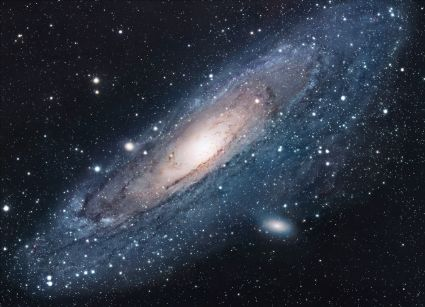
\includegraphics[scale=1.7]{universe}
\caption{The Universe}
\label{fig:universe}
\end{figure}